\chapter{Falling into Sagittarius A*}
\label{ch:xinfall}

The last capability of the simulator is the one most often asked of a black
hole: what would someone falling in see and feel? None of it is a matter of
taste. The light, the clocks and the tides follow from the metric, and this
chapter computes each of them for \sgra{} ($\astar = 0.94$) along one
physical worldline. The fall is rendered live with every effect on.

\section{The trip}

\emph{Worldline.} A free fall is a timelike geodesic of the same Hamiltonian
the ray tracer uses, $H = \frac12 g^{\mu\nu} p_\mu p_\nu$, with $H = -\frac12$
in place of 0, so the affine parameter is the proper time $\tau$ of the
faller. It is integrated in double precision (Dormand--Prince, tolerance
$10^{-12}$) in the \emph{ingoing} Kerr--Schild chart (Chapter~\ref{ch:xks}),
which is regular across the future horizon where Boyer--Lindquist
coordinates fail. The default start is \emph{rain}: an observer dropped from
rest at infinity ($E = 1$, $L_z = 0$, $Q = 0$), whose polar angle stays
constant, the ``river'' frame of \citet{HamiltonLisle2008}. The trip begins at
$r_0 = \XIfRzero\,M$ at a polar angle of $\XIfTheta\degr$. A release
from rest relative to the local ZAMO is the alternative start.

\emph{Where it stops.} The trip ends just above the inner (Cauchy) horizon,
at $r = \XIfRstop\,M$ ($r_- = \XIfRminus\,M$). Perturbations falling in pile
up at the inner horizon and drive the mass inflation of
\citet{PoissonIsrael1990}, so the classical Kerr interior beyond it is not a
reliable description of a real black hole. The simulator says so on screen
rather than render it.

\emph{Checks.} In Schwarzschild the worldline reproduces the closed forms for
both starts: the cycloid of a fall from rest, and
$\tau = \frac23 (r_0^{3/2} - r^{3/2})/\sqrt{2M}$ for rain. The proper time to
$r = 2M$ matches them to $\XIfSchwErr$, and unit tests check radii inside the
horizon as well. For $\astar = 0.94$, across the $\XIfNsamples$ steps of the
default trip through $r_+$, $L_z$ and $Q$ are conserved to $\XIfMaxdL$ and
$\XIfMaxdQ$, and the norm of the 4-velocity to $\XIfMaxNorm$; $E = -p_t$ is
constant by construction. $Q$ is reconstructed through Boyer--Lindquist
components, so it is checked away from the two horizons, and it uses Carter's
constant for timelike geodesics. The tracer's existing routine assumed light;
this chapter generalised it.

\emph{Camera.} The faller's frame takes $e_0 = u$ and builds its three spatial
legs by Gram--Schmidt, with the full metric, from the Kerr--Schild coordinate
directions $\partial_r$, $\partial_\theta$, $\partial_\phi$ projected
orthogonal to $u$. Those directions are smooth through $r_+$ in this chart, so
the camera is too, and the legs mirror the exterior observers' triad, so
looking around works exactly as in Chapter~\ref{ch:xobs}.

\emph{Light.} The live renderer traces the same backward rays as before,
switched to the ingoing chart. One thing changes: what ``captured'' means.
Traced backward from inside $r_+$, every ray leaves outward through the future
horizon, because the light came in from outside. A backward ray that heads
inward from outside, by contrast, is bound for the \emph{past} horizon, which
this chart reaches only as $t \to -\infty$; such rays carry no light in this
model. The CPU twin applies the same rule. On $\XIfGpuStrips$ image strips
through the centre of the faller's view, at radii from $6\,M$ to $0.9\,M$
(two of them inside the horizon), the edges of the dark region in the live
image agree with the double-precision tracer within $\XIfGpuMaxPx$ pixels.
Across the horizon itself the image evolves smoothly. Between full frames at
$r_+ + 0.03\,M$ and $r_+ + 0.01\,M$, $\XIfContOut$ per cent of the pixels
change between dark and sky; across $r_+$, from $r_+ + 0.01\,M$ to
$r_+ - 0.01\,M$, $\XIfContAcross$ per cent; and inside, from $r_+ - 0.01\,M$
to $r_+ - 0.03\,M$, $\XIfContIn$ per cent.

\section{Time}

From $r_0$, the faller reaches the ergosphere ($r_E = \XIfRergo\,M$ at this
latitude) after $\tau = \XIfTauErgo\,M$ of proper time, and the horizon after
$\XIfTauHor\,M$: $\XIfTauHorMin$ minutes for \sgra{}, whose unit of time is
$GM/c^3 = \XIfTg$\,s. Only $\XIfTauErgoHorSec$\,s pass between entering the
ergosphere and crossing the horizon. From the horizon to the end of the model
just above $r_-$ takes $\XIfTauInside\,M$, or $\XIfTauInsideSec$\,s.

Far-away time behaves very differently (Fig.~\ref{fig:xfallreadouts}, left).
The Boyer--Lindquist time $t$ of a distant clock grows without bound as the
faller approaches $r_+$, so a distant observer never sees the crossing. The
faller's own clock notices nothing, and the Kerr--Schild time stays finite.
Inside, $t$ is no longer a time at all: no signal sent from there can reach
the outside.

\section{What you see}

Figure~\ref{fig:xfall} shows the view straight ahead, at the hole, with the
Milky Way panorama as the distant sky (the hypothetical thin disk is switched
off: \sgra{} has none). Far out, the shadow sits in the lensed Milky Way. As
the faller speeds up, aberration and the Doppler shift crowd the sky toward
the direction of motion and blueshift it, and the shadow swells until, near
$r_+$, it fills most of the view ahead. Crossing the horizon is a non-event
locally. The frames on either side of it differ smoothly, with no seam or
flash, as the regular chart demands. Inside, the outside universe is still
there. Behind the faller it fills the whole view, redshifted and dimmed
(below). Ahead it survives only as a band at the edge of the view. The dark
region ahead is light that would come from the past horizon, from no source
in this model.

The colour of that light changes along the way, and it depends on direction.
Ahead, the light that skims the edge of the dark region is blueshifted: it
arrives at $\XIfEdgeSixMin$--$\XIfEdgeSixMax$ times its frequency at infinity
at $6\,M$, up to $\XIfEdgeTwoMax$ times at $2\,M$, and up to
$\XIfEdgeZeroNineMax$ times at $0.9\,M$, inside the horizon. Behind, the
faller is running away from the light, and it is redshifted: it arrives at
$\XIfFreqBehindStart$ times its frequency at infinity at the start,
$\XIfFreqBehindHor$ times at the horizon and $\XIfFreqBehindEnd$ times at the
end of the trip. Light from the side arrives at $\XIfFreqSideHor$ times its
frequency at infinity at the horizon (Fig.~\ref{fig:xfallreadouts}, middle).

\begin{figure}
\centering
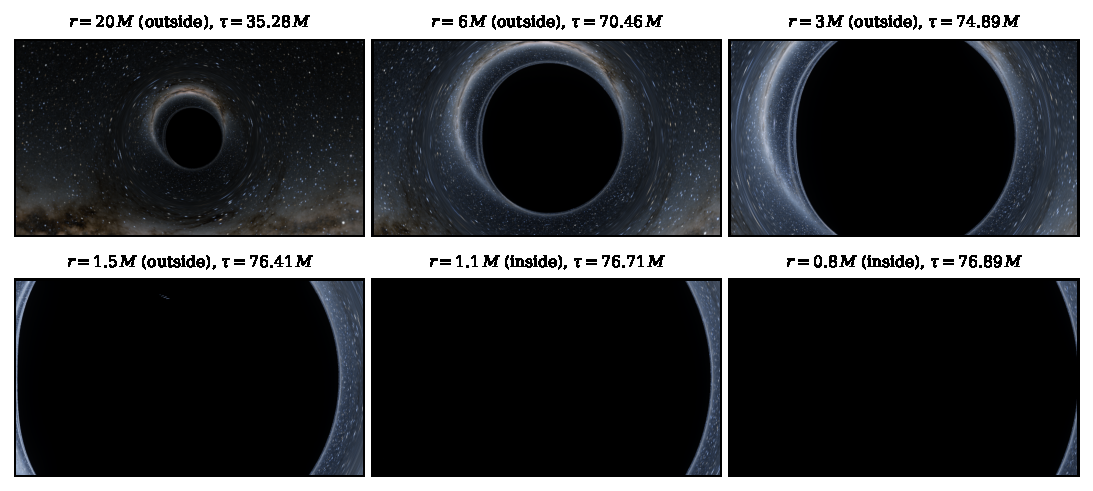
\includegraphics[width=\textwidth]{figures/fig_x_fall.pdf}
\caption{Falling into \sgra{} ($\astar = 0.94$): the view straight ahead of an
observer dropped from rest at infinity, at polar angle $\XIfTheta\degr$, live
GPU renders of the double-precision worldline (field of view 1.6\,rad; the
lensed Milky Way is the only light). Top: outside the horizon
($r_+ = \XIfRplus\,M$); bottom: just outside it and inside it. Labels give
the radius and the faller's proper time since $r_0 = \XIfRzero\,M$.}
\label{fig:xfall}
\end{figure}

\section{Tides}

The tidal field felt by the faller is the electric part of the Riemann tensor
in its own frame, $E_{ij} = R_{i\alpha j\beta} u^\alpha u^\beta$: two free
particles separated by $\xi$ accelerate apart at $-E_{ij}\xi^j$. The simulator
computes it exactly from the analytic metric. The Christoffel symbols come
from complex-step derivatives, and their derivatives from central differences.
It is checked in two ways. In Schwarzschild it reproduces the radial-fall
values $-2M/r^3$ and $M/r^3$, also inside the horizon. And everywhere on the
trip $8(E_{ij}E^{ij} - B_{ij}B^{ij})$ equals the closed-form Kretschmann
scalar of Kerr to $\XIfKretErr$.

\sgra{} is gentle. Across a 2\,m body, the tidal stretch is
$\XIfStretchHor$\,m\,s$^{-2}$ at the horizon and $\XIfStretchEnd$\,m\,s$^{-2}$
at the end of the trip (Fig.~\ref{fig:xfallreadouts}, right). Tides scale as
$M/r^3$, and the horizon radius scales with $M$, so at the horizon they fall
as $1/M^2$. A black hole of four million solar masses can be entered intact;
a stellar-mass one could not be.

\begin{figure}
\centering
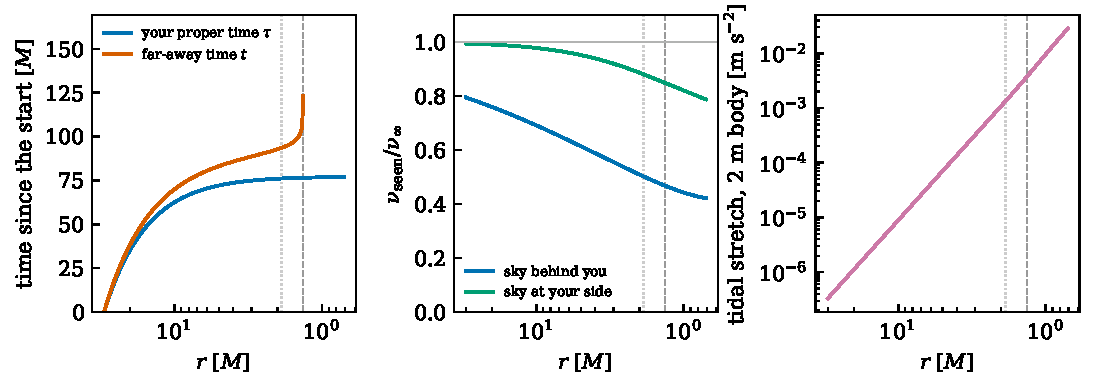
\includegraphics[width=\textwidth]{figures/fig_x_fall_readouts.pdf}
\caption{The faller's instruments along the trip (dashed: the horizon; dotted:
the ergosphere at this latitude). Left: its proper time and the far-away
time, which diverges at $r_+$. Middle: frequency of the sky light arriving
from straight behind and from the side, relative to its frequency at
infinity. Right: tidal stretch across a 2\,m body.}
\label{fig:xfallreadouts}
\end{figure}

\section{Limits}

The fall is classical, vacuum Kerr, along one geodesic. The accretion flow,
the hypothetical disk and every quantum effect are left out, and the trip
stops at the inner horizon by design. The sky is the panorama seen from Earth,
used as the distant background, as in the rest of this report. The camera
frame is one choice among many: another tetrad rotates or boosts the view but
changes no physics.
